\section{Configurable Systems}\label{ch:configurable-systems}
\theoremstyle{definition}
\newtheorem{definition}{Definition}[section]

In this section, we explain the general concepts behind configurable software systems and the benefits and challenges when using them. 

We explain what a feature and a configuration is in the context of configurable software systems in \autoref{feature-config}. 
We introduce functional and non-functional properties in \autoref{ch:properties} and highlight differences between them.

\subsection{General Concepts}\label{ch:general-concepts}
%What is a Conf. system and why we use it
We call a system configurable if it offers options that allow developers and end-users to turn functionality on and off.
This gives the system the benefit of satisfying the demand of multiple user groups by providing a single software system containing various features
~\cite{TooManyKnobs}.


\begin{figure}[h]
    \centering
    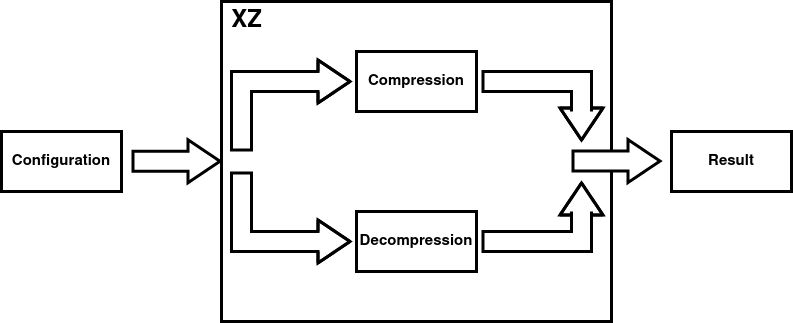
\includegraphics[scale=0.55]{gfx/ConfigurableSystemXZ.png}
    \caption{Simplified version of \textsc{XZ}.}
    \label{fig:xz}
\end{figure}

%Example for such a system using xz
As an example, let us inspect the compression tool \textsc{XZ}\footnote{Visited at 21.03.2023 \url{https://tukaani.org/xz/}}.
In \autoref{fig:xz} depicts a simplified version of \textsc{XZ}, which contains two main functions, encryption, and decryption. 
It is up to the user to decide what he needs, but regardless of his choice, a single software system contains both functions.

\subsection{Features and Configurations}\label{feature-config}

%What is a feature
During the years there have been many definitions to what a \emph{feature} is, on one side, features are used as a means of communication between
the different stakeholder of a system, where on the other hand, a feature is defined as an implementation-level concept. 
To unify both applications Apel et.al. introduced the following definition~\cite{Feature-Oriented-Software-Product-Lines}:

%Definition
\begin{definition}
    "A structure that extends and modifies the structure of a
    given program in order to satisfy a stakeholder's requirement, to implement and
    encapsulate a design decision, and to offer a configuration option."     
\end{definition}

%Example of feature on xz an definition of configuartion
Thus, a feature is both an abstract concept that refers to particular functionality of a system and the implementation of that functionality.
In our example \autoref{fig:xz} both, \textit{Compression} and \textit{Decompression}, are unique features, they refer to a piece of functionality of the system and the
implementation. 

%Numeric and binary feature
We differentiate between \emph{binary} features \emph{numeric} features. A binary feature can be either selected or deselected; 
commonly, we denote a binary feature with $1$ if we select it and $0$ otherwise. 
We denote a numeric feature with a numerical value; these can have various meanings depending on the feature it implements. 
For \autoref{fig:xz}, \textit{Decompression} could be a binary feature since we either have the option to decrypt a file or not; on the contrary, 
\textit{Compression} could be implemented as a numeric feature, where the numeric value represents the quality of compression we want. 

%What is a Configuration option
A configuration option is a predefined way for developers to change the functionality of the configurable system; 
these options allow us to select features we want to include or exclude. Thus, a configuration is a set of configuration options, whereas 
we call a configuration valid as long as it satisfies the system's constraints.

%What is a Configuration space
The configuration space refers to the set of all configurations. However, some of these configurations are invalid. 
In practice, we cannot execute systems with invalid configurations. 
Therefore, we shall implicitly exclude all invalid configurations whenever we refer to a configuration space.

%Example
As an example, \textsc{XZ} offers the user different features such as \textit{Compression} and \textit{Decompression}, whereas 
the configuration options \textit{0-9} specify the degree of compression. An invalid configuration would be to select multiple 
degrees of compression.

\section{Functional and Nonfunctional Properties}\label{ch:properties}

When analyzing a configurable system we can divide the properties of that system into two categories, functional and non-functional properties.
As functional properties 
